
\begin{figure}[t]
    \centering
    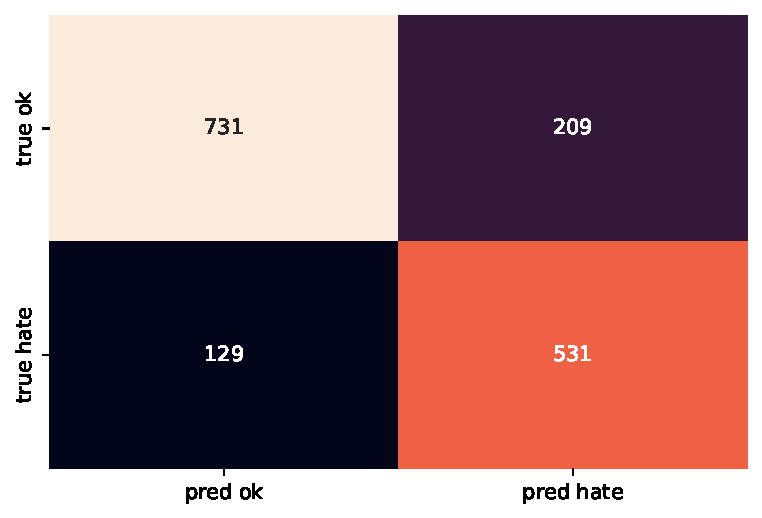
\includegraphics[width=0.5\textwidth]{img/hateval_confusion_matrix.pdf}
    \caption{Error analysis of the model}
    \label{fig:hateval_error_analysis}
\end{figure}


Para tener una mejor idea de lo ocurrido con nuestros clasificadores, realizamos un análisis de error sobre los datasets en español. Para intentar mitigar los efectos de la varianza de los clasificadores, tomamos las salidas de 10 clasificadores BETO entrenados con una distinta semilla y analizamos el error sobre un clasificador de ensamble por voto mayoritario; de esta manera, tratamos de buscar aquellos errores frecuentes, aquellos que la mayoría de los 10 clasificadores erran. Nos centraremos en observar los errores de la etiqueta HS, y particularmente veremos qué pasa con los falsos positivos. La figura \ref{fig:hateval_error_analysis} muestra la matriz de confusión de nuestros clasificadores. Como era de esperar (dado que la precisión es más baja que la sensitividad) tenemos muchos falsos positivos, por lo cual haremos eje en observar estos errores.


\begin{table}[t]
    \small
    \begin{tabularx}{\columnwidth}{l X}
        Índice   &  Tweet \\
        \hline
        1   & Una cosa que le pasó a una amiga mexicana en Barcelona. Una chica repartía flyers en castellano y catalán, le dio uno a mí amiga en catalán y al segundo se lo quitó y se lo dio en castellano. -No, déjalo que entiendo catalán -Ah, es que como te he visto cara de sudaca Racismo 0 URL \\
        2   & Los fascistas salen de la ratonera para atacar a los 100 inmigrantes que han logrado saltar la valla de Ceuta. Asco de prensa y partidos políticos que se pelean por lograr los votos de los fascistas. Ningún ser humano es ilegal. \\
        3   & @saludhernandezm Esas personas que extrañan dictaduras, cualquier dictadura, aún más si son las ibéricas que ponen como eje a Madrid; su cultura, política e idioma sobre la idiosincrasia de los demás. Esos mismos que añoran a Franco y viven en un país 'Sudaca' creyéndose dueños de la verdad.	 \\
        4   & @caciena después sigo siendo un sudaca pero bueno \\
        5   & @ArturoMonteduro Pues tienes toda la razón del mundo. Y lo peor es que seguro que tenía papeles y DNI español, pero queda mejor decir "argelino" o "uno d'estos del top manta", "puto inmigrante", o "moro mierda" y ya pues matas dos pájaros de un tiro. \\
        6   & Obvio me ofendo cuando algn Sudaca hace algn comentario presuponiendo que los mexicanos somos feos, o que el pas est de la verga. Entre mexicanos podemos hablar mierda de Mxico, pero que a ningn pinche extranjero se le ocurra, porque va a haber pedo! \\
        7   & TODOS LOS INMIGRANTES Y GITANOS FUERA!!! Menos: el colombiano que me vende coca, el negro que me consigue putas, el moro que me pasa costo y el gitano que me vende maría. \\
        8   & Ayer nos fuimos a tomar algo con los cumpas: Dos españoles, un ponja, un africano y un sudaca. Estamos para campaña de United Colours of Benneton. \\
        \hline
    \end{tabularx}

    \caption{Falsos positivos del modelo de clasificación para la detección de discurso de odio (HS).}
    \label{tab:hateval_error_analysis}
\end{table}


En la tabla \ref{tab:hateval_error_analysis} podemos observar algunos de los errores que comete nuestros clasificador. Por un lado, podemos observar que algunos errores se deben a cierto overfitting a ciertas palabras ``clave'' (como las nro. 1, 2 y 3) muchas de las cuales son producto del proceso de recolección que está fuertemente basada en keywords (inmigrante, sudaca, por ejemplo). Haciendo un poco de probing en los clasificadores, podemos ver que ciertas palabras como ``sudaca'' o ``migrante'' automáticamente disparan una salida positiva en discurso de odio \footnote{Puede probarse esto en el cuadro interactivo de \url{https://huggingface.co/pysentimiento/robertuito-hate-speech?text=migrante}. Si bien este modelo es el que presentaremos en el capítulo \ref{chap:07_domain_adaptation}, el problema se mantiene}. Otros de los casos que nuestros clasificadores no parecieran detectar son los reportes de discriminación (como el caso 5, parcialmente también el 1) o casos de apropiación cultural (caso 3 o 5) o contenido irónico (casos 3, 4, 7 y 8 ). Estos casos dan cuenta de la dificultad de la detección de esta tarea.


\begin{table}[t]
    \small
    \centering
    \begin{tabularx}{\textwidth}{l X}
        Índice &  Tweet \\
        \hline
        1 &Callate la puta boca pesada @Lauu\_tb \\
        2 & me cansada tía cállate ya la puta boca lo que te queda de vid \\
        3   & FLOR SALTANDO AHÍ LA RE PUTA MADRE TE LO MERECES PEDAZO DE FORRA TE LO MERECES, EN LA CARA DE TODOS HIJA ASÍ SE HACE \\
        4   & Callate! cerra el orto un ratooo! es mas, no te queres morir mejor? la puta que te pario  \\
        5   & Esta mujer es lo más la puta madre URL\\
        %5   & @nlopezi\_ Imbécil tu puta prima! Gilipollas! Estúpida \\
        6   & @csdb530 @carvasar Claro, porque la culpa la tienen las niñas embarazadas y las víctimas de acoso sexual, violación... URL \\
        7   & \#Pendejos Don't call me gringo You fuckin beaner Stay on your side Of that goddamn river Don't call me gringo You beaner No me digas beaner Mr. puñetero Te sacaré un susto Por racista y culero No me llames frijolero Pinche gringo puñetero \\
        8   & Mónica que te calles la puta boca \#OTGala7 \\
        9   & @pablocasado\_ @imbrodamelilla @TeoGarciaEgea pablo no quieren concertinas , un muro de 12 metros o mas de altura de dos plantas de pisos ,se acabo los problemas @guardiacivil @policia @EMADmde @MonarquiaEspana nadie se quejaría de nada \\
        10   & \#OTGala7 Noemí JAJAJAJAJAJA ESTA MUJER ES LA PUTA AMA \\
        \hline
    \end{tabularx}
    \caption{Ejemplos mal etiquetados como discurso de odio. En etiqueta marcamos cómo están etiquetados (erróneamente). El índice es meramente para referencia.}
    \label{tab:hateval_label_errors}
\end{table}


Algo que observamos también es que hay una fuerte cantidad de errores de etiquetado. La tabla \ref{tab:hateval_label_errors} muestra algunos de estos ejemplos, todos estos etiquetados incorrectamente como discurso de odio. Si bien es difícil establecer una causa específica para cada uno de estos errores, es posible que sean causados por una combinación de:

\begin{itemize}
    \item Confusión entre lenguaje ofensivo y discurso de odio (ejemplos 1, 2, 3, 4 y quizás 5)
    \item Desconocimiento cultural (ejemplo 7, quizás 10 también)
    \item Opinión pero no necesariamente discurso de odio (ejemplo 9)
    \item Tweets truncados (el ejemplo 6 fue mal recolectado y está truncado)
\end{itemize}


\begin{table}
    \small
    \begin{tabularx}{\textwidth}{l X}
        Etiqueta      & Tweet \\
        \hline
        \mr{13}{No HS} & - @ArturoMonteduro Pues tienes toda la razón del mundo. Y lo peor es que seguro que tenía papeles y DNI español, pero queda mejor decir ``argelino'' o ``uno d'estos del top manta'', ``puto inmigrante'', o ``moro mierda'' y ya pues matas dos pájaros de un tiro.      \\
                      & @UbedaJoseA @WalkingDead\_AMC Perro cállate ala puta       \\
                      & @iancandado Es sudaca como.tu       \\
                      & @Stopfalsasdenun Pero que tienes en la cabesaaaa?(con voz de sudaca de mierda)       \\
                      & @\_Lassana\_ Me la has puesto como un tanque apuntando a un campanario negrata		       \\
                      & @odiomistweets Es una analogía pendejo sudaca	       \\
                      %& @MifasolMaite Sudaca? K racista eres \\
                      & @ElQuemaMarias te parece que un sudaca tatuado excelentemente bien dotado y carismático no es buen ejemplo?       \\
                      & @HQGatica @AnglicaVillarN1 Este sueco con cara de bolita .xq eso es este aspiracional desclasado . x dignidad debería irse . no lo hará xq este sudaca no la tiene !!!       \\
                      %& @SOFIAGAVIRIAC Ambas cosas y Sudaca (lo que eso signifique)       \\
                      & @SleeplessXenn @envdiaN Este finde te recojo y vamos al barrio negrata de envdian       \\
                      & @elmundoes El q quería quitar concertinas y luego quitarse a los inmigrantes !!       \\
                      & @AlexTor1975 @sanchezcastejon Disfràcese de moro o negro, y al momento tiene resuelto el problema de espera, de verdad, mano de santo!. Nada como ser invasor, refugiado, o inmigrante en este paraíso terrenal. Ahora, si eres nativo del paraíso!!!!, Se te puede complicar la existencia!!!!. \\
        \hline
        \mr{2}{HS}    & CALLATE YA Y HAZME LA PUTA CENA JODERRR URL \\
                      & Basta ya de buenismo, si te no respetas a la polica ni a la guardia civil en la frontera nada de concertinas, simplemente 4 tiros. Fin del problema \\
                      & @benemeritosGC La solución es fácil, muro de hormigón de 3 metros de alto, garitas cerradas para vigilancia y por delante la valla actual con concertinas. No es caro, es cuestión de quererlo hacer. \\
                      & Por desgracia, no queda otra, aportan poco y nos cuestan mucho. Incluido nuestra seguridad. \#Inmigración \#Immigration URL \\
        \hline
    \end{tabularx}
    \caption{Algunos ejemplos observados en el análisis de error que carecen de contexto conversacional. Etiqueta es la asignada en el dataset}
    \label{tab:hateval_lack_of_context}
\end{table}


Dentro de estas asignaciones posiblemente erróneas, en el análisis de error separamos un subconjunto especial sobre el cual entendemos que falta contexto para asignar una etiqueta. Si bien esto a veces puede ser inferido por un humano (por ejemplo, infiriendo que un comentario habla de tal o cual suceso), un algoritmo de detección podría beneficiarse de esta información. Para el dataset en concreto, muchos de estos comentarios tienen un contexto implícito: muchos hablan de incidentes en la frontera de Ceuta (España) entre inmigrantes y la policía, debido al proceso de recolección realizado. La tabla \ref{tab:hateval_lack_of_context} muestra algunos de estos ejemplos. En algunos ejemplos podemos observar que falta contexto conversacional: aquellos donde tenemos un @username al principio del tweet indican que son una respuesta. En otros casos, falta información de un suceso o noticia sobre la que se está comentando: los que terminan con URL suelen ser citas de otros tweets o links a noticias.



